\section{The Main Evaluation Datasets and Challenges}

In this thesis, we will review the Text-to-SQL Challenges and datasets and structure of existing datasets and difference between them. Datasets to be covered are: ATIS, GeoQuery, IMDb, Advising, WikiSQL, Spider.

\subsubsection{ATIS (Air Travel Information System) Dataset}

A relational schema is used to organize data from the official airline guide in the ATIS corpus. There are 25 tables containing information about fares, airlines, flights, cities, airports, and ground services. All questions related to this dataset can be answered using a single relational query. The relational database uses shorter tables for this dataset to answer queries intuitively.

% Here is an example query from the ATIS dataset: Input is in natural language, and the output is in \lambda calculus.
% \begin{figure}[htb]
%     \centering
%     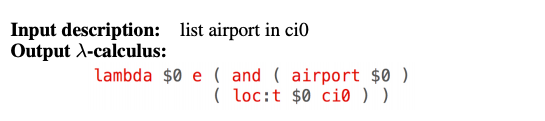
\includegraphics[width=0.8\textwidth]{pics/db/ATIS.png}
%     \caption{Example from ATIS dataset for semantic parsing}
%     \label{fig:ATIS}
% \end{figure}

\subsubsection{GeoQuery Dataset}

United States geography is represented in the Geoquery dataset. About 800 facts are expressed in Prolog. State, city, river, and mountain information can be found in the database. Geographic and topographical attributes such as capitals and populations make up the majority of the attributes.

\subsubsection{IMDb Dataset}

The IMDb dataset contains 50K reviews from IMDb. There is a limit of 30 reviews per movie\cite{maas-EtAl:2011:ACL-HLT2011}. Positive and negative reviews are equally represented in the dataset. The dataset creators considered a negative review with a score of 4 out of 10 and a positive review with a score of 7 out of 10. When creating the dataset, neural reviews are not taken into account. Furthermore, Training and testing datasets are equally divided.

\begin{figure}[htb]
    \centering
    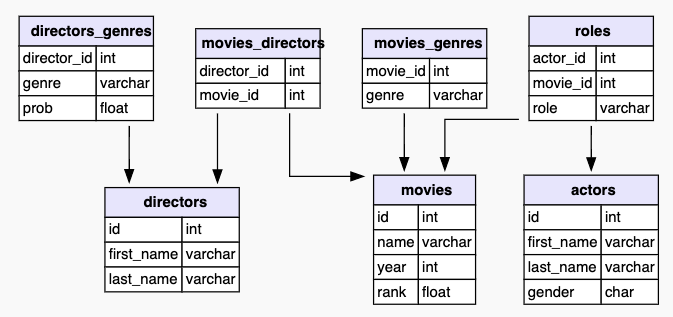
\includegraphics[width=0.8\textwidth]{pics/db/IMDb.png}
    \caption{Database Structure of IMDb dataset}
    \label{fig:IMDb}
\end{figure}

\newpage % to avoid page break

\subsubsection{Advising Dataset}

The Advising dataset was created in order to propose improvements in text2SQL systems. The creators of the dataset compare human-generated and automatically generated questions, citing properties of queries that relate to real-world applications. Dataset consists of questions from university students about courses that lead to particularly complex queries. The database contains fictional student records. The dataset includes student profile information, such as recommended courses, grades, and previous courses. In an academic advising meeting, students were asked to formulate questions they would ask if they knew the database. Many of the queries in this dataset were the same as those in ATIS, GeoQuery, and Scholar.

\begin{figure}[htb]
    \centering
    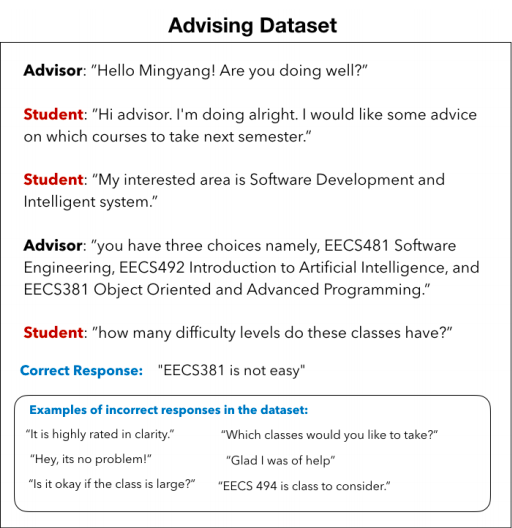
\includegraphics[width=0.5\textwidth]{pics/db/Advising.png}
    \caption{Example from Advising dataset \cite{vig_comparison_2019}}
    \label{fig:Advising}
\end{figure}

\subsubsection{WikiSQL Dataset}

WikiSQL consists of 80K+ natural language questions and corresponding SQL queries on 24K+ tables extracted from Wikipedia. Neither the train nor development sets contain the database in the test set. Databases and SQL queries have simplified the dataset's creators' assumptions. This dataset consists only of SQL labels covering a single SELECT column and aggregation and WHERE conditions. Furthermore, all the databases contain only one table.

The database does not include complex queries involving advanced operations like JOIN, GROUP BY, ORDER BY, etc. Prior to the release of SPIDER, this dataset was considered to be a benchmark dataset. Using WikiSQL has been the subject of a great deal of research. WikiSQL's "WHERE" clause has been recognized as one of the most challenging clauses to parse semantically, and SQLNet and SyntaxSQL were previous state-of-the-art models.


\begin{figure}[htb]
    \centering
    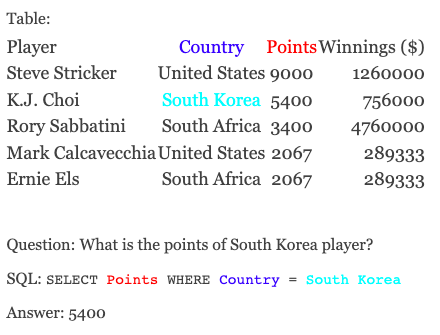
\includegraphics[width=0.5\textwidth]{pics/db/WikiSQL.png}
    \caption{Example from WikiSQL dataset\cite{hwang_comprehensive_2019}}
    \label{fig:WikiSQL}
\end{figure}

\subsubsection{WikiSQL Challenge}

The WikiSQL challenge is a research competition focused on developing natural language interfaces for databases. The challenge includes several state-of-the-art Text-to-SQL solutions proposed by different research teams.

One example of a state-of-the-art Text-to-SQL solution in the WikiSQL challenge is the Seq2SQL model, which uses a sequence-to-sequence learning framework to map natural language input to SQL queries. The model uses an attention mechanism to align the input and output sequences and a pointer network to handle SQL queries with complex structural dependencies.

Another example is the Spider model, which uses a combination of recurrent and convolutional neural networks to learn the mapping between natural language and SQL queries. The model uses a hierarchical structure to process the natural language input, with separate modules for understanding the query's intent, columns, and constraints.
One difference between these research approaches is the specific deep learning architecture used. The Seq2SQL model uses a sequence-to-sequence framework, while the Spider model uses a combination of RNNs and convolutional neural networks. Additionally, the Spider model uses a hierarchical structure to process the natural language input, while the Seq2SQL model processes the input linearly.

Another difference is in the evaluation metrics used. The Seq2SQL model is evaluated using the execution accuracy of the generated SQL queries, while the Spider model is evaluated using a combination of execution accuracy and natural language understanding metrics.
Overall, both the Seq2SQL and Spider models are state-of-the-art Text-to-SQL solutions that have achieved high performance in the WikiSQL challenge. However, their specific architectures and evaluation metrics differ, which can affect their performance and accuracy on different tasks.

\subsubsection{Spider Dataset}

Yale University students created this dataset.
The SPIDER database contains 10K questions and 5K+ complex SQL queries covering 138 different domains across 200 databases. As opposed to previous datasets (most of which used only one database), this one incorporates multiple datasets. Creating this corpus was primarily motivated by the desire to tackle complex queries and generalize across databases without requiring multiple interactions.

\begin{figure}[htb]
    \centering
    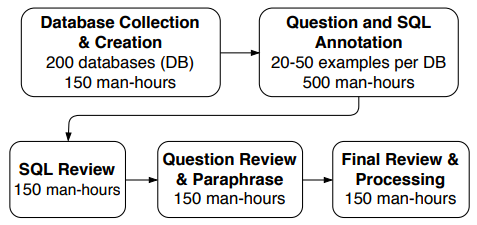
\includegraphics[width=0.6\textwidth]{pics/db/Spider.png}
    \caption{Example from Spider dataset\cite{yu_spider_2019}}
    \label{fig:Spider}
\end{figure}

Creating a dataset involves three main aspects: SQL pattern coverage, SQL consistency, and question clarity. Several databases from WikiSQL are included in the dataset. The table is complex as it links several tables with foreign keys. In SPIDER, SQL queries include: SELECT with multiple columns and aggregations, WHERE, GROUP BY, HAVING, ORDER BY, LIMIT, JOIN, INTERSECT, EXCEPT, UNION, NOT IN, OR, AND, EXISTS, LIKE.

\begin{figure}[htb]
    \centering
    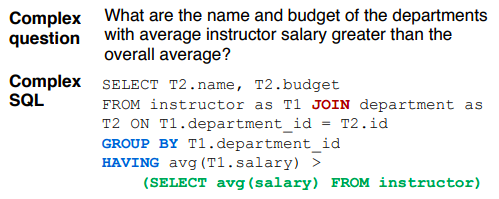
\includegraphics[width=0.8\textwidth]{pics/db/Spider2.png}
    \caption{Example of Question-Query set from SPIDER\cite{yu_spider_2019}}
    \label{fig:Spider2}
\end{figure}

SPIDER's exact matching accuracy was 12.4\% compared to existing state-of-the-art models. As a result of its low accuracy, SPIDER presents a strong research challenge. Current SPIDER accuracy is around 75.5\% with an exact set match without values (refers to values in the WHERE clause) and around 72.6\% with values.

\subsubsection{Spider Challenge}

The SPIDER challenge is a research competition dedicated to developing cutting-edge Text-to-SQL solutions. In this challenge, participants strive to develop algorithms that can automatically generate structured SQL queries from natural language input, to improve the performance and accuracy of Text-to-SQL models.

In the SPIDER challenge, numerous state-of-the-art Text-to-SQL solutions have been proposed, such as the Spider model. This model uses a combination of recurrent and convolutional neural networks to learn the mapping between natural language and SQL queries. This model also has a hierarchical structure, which allows it to process the natural language input more effectively, thereby allowing it to handle complex queries and variations in language with greater precision and accuracy. This model successfully generates accurate and efficient SQL queries from natural language inputs.

One difference between the SPIDER and WikiSQL challenges is the specific dataset that is used for evaluation. The SPIDER challenge uses a dataset of complex SQL queries and natural language questions derived from real-world databases, while the WikiSQL challenge uses a dataset of more straightforward SQL queries and natural language questions derived from Wikipedia articles. This difference in the dataset can affect the performance and accuracy of the models on the different tasks.

Another difference is in the evaluation metrics used. The SPIDER challenge evaluates the models using execution accuracy and natural language understanding metrics, while the WikiSQL challenge evaluates the models using only execution accuracy. This difference in the evaluation metrics can affect how the models are trained and their performance on the tasks.